\chapter*{Копии экранов моделирования исходного проекта VINC (исходная программа)}
\addcontentsline{toc}{chapter}{Копии экранов моделирования исходного проекта VINC(исходная программа)}

По умолчанию, в диаграмму (которую необходимо получить в приложении Vivado) добавлены сигналы шины AXI4 MM, представляющие собой 5 независимых каналов передачи сообщений, которые представлены в таблице \ref{tab:t1}.

\begin{table}[h]
	\begin{center}
		\captionsetup{singlelinecheck = false, justification=raggedright}
		\caption{\label{tab:t1}Результаты замеров времени.}
		\begin{tabular}{|c|c|}
			\hline
			Канал передачи & Группы сигналов \\
			\hline
			Канал чтения адреса от ведущего к ведомому & m00\_axi\_ar* \\
			\hline
			Канал чтения данных от ведомого к ведущему & m00\_axi\_r* \\
			\hline
			Канал записи адреса записи от ведущего к ведомому & m00\_axi\_aw* \\
			\hline
			Канал запись данных от ведущего к ведомому & m00\_axi\_w* \\
			\hline
			Канал записи ответа от ведомого к ведущему & m00\_axi\_b* \\
			\hline
		\end{tabular}
	\end{center}
\end{table}

Каналы позволяют сформировать конвейерные транзакции чтения и записи. Последовательность событий транзакции чтения можно представить следующим образом: ARVALID→ ARREADY→ RVALID→ RREADY.

На рисунке \ref{png:read_data_1} приведена транзакция чтения данных вектора на шине AXI4 MM из DDR памяти.
\begin{figure}[H]
	\centering{
		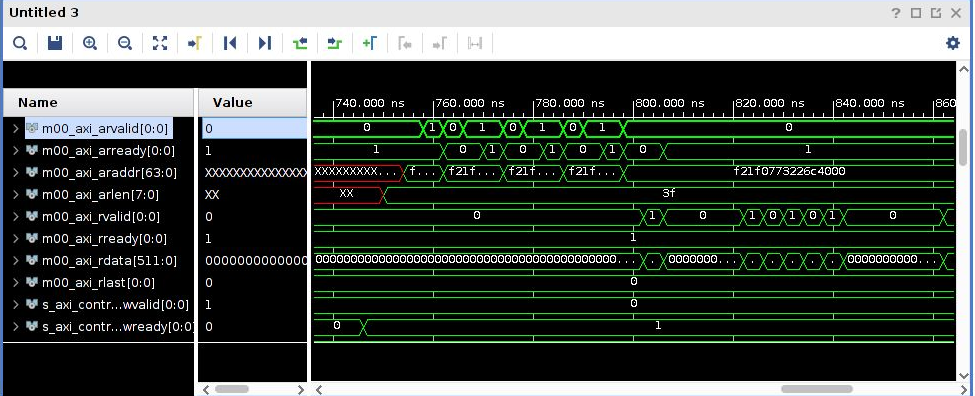
\includegraphics[scale=0.8]{images/diagram_ar_r_1}
		\caption{Транзакция чтения данных вектора на шине AXI4 MM из DDR памяти}
		\label{png:read_data_1}
	}
\end{figure}

Последовательность событий транзакции записи: AWVALID→ AWREADY → WVALID → WREADY → BVALID → BREADY.

На рисунке \ref{png:write_data_1} приведена транзакция записи результата инкремента данных на шине AXI4 MM.
\begin{figure}[H]
	\centering{
		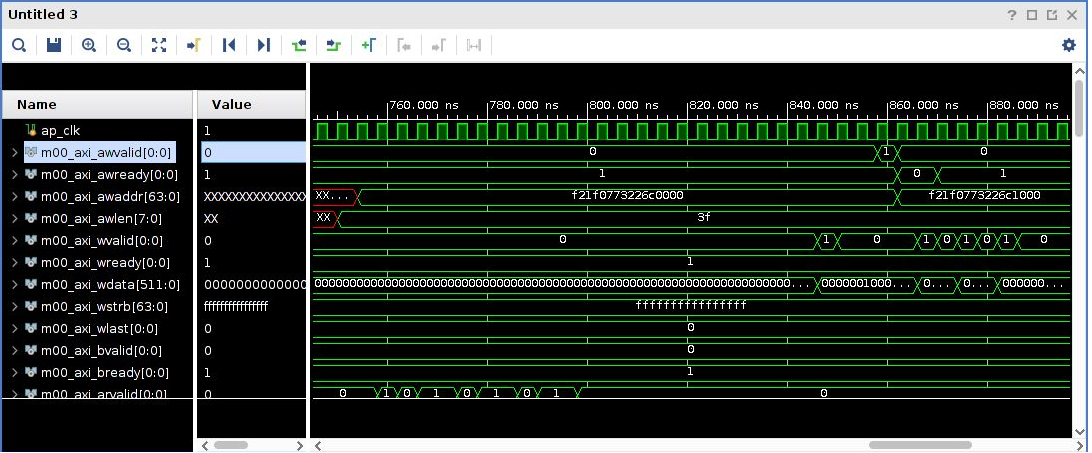
\includegraphics[scale=0.7]{images/diagram_aw_w_1}
		\caption{Транзакция записи результата инкремента данных на шине AXI4 MM}
		\label{png:write_data_1}
	}
\end{figure}

На рисунке \ref{png:increment} приведен фрагмент кода модуля rtl\_kernel\_wizard\_0\_example\_adder.v с выполнением инкрементирования данных.
\begin{figure}[H]
	\centering{
		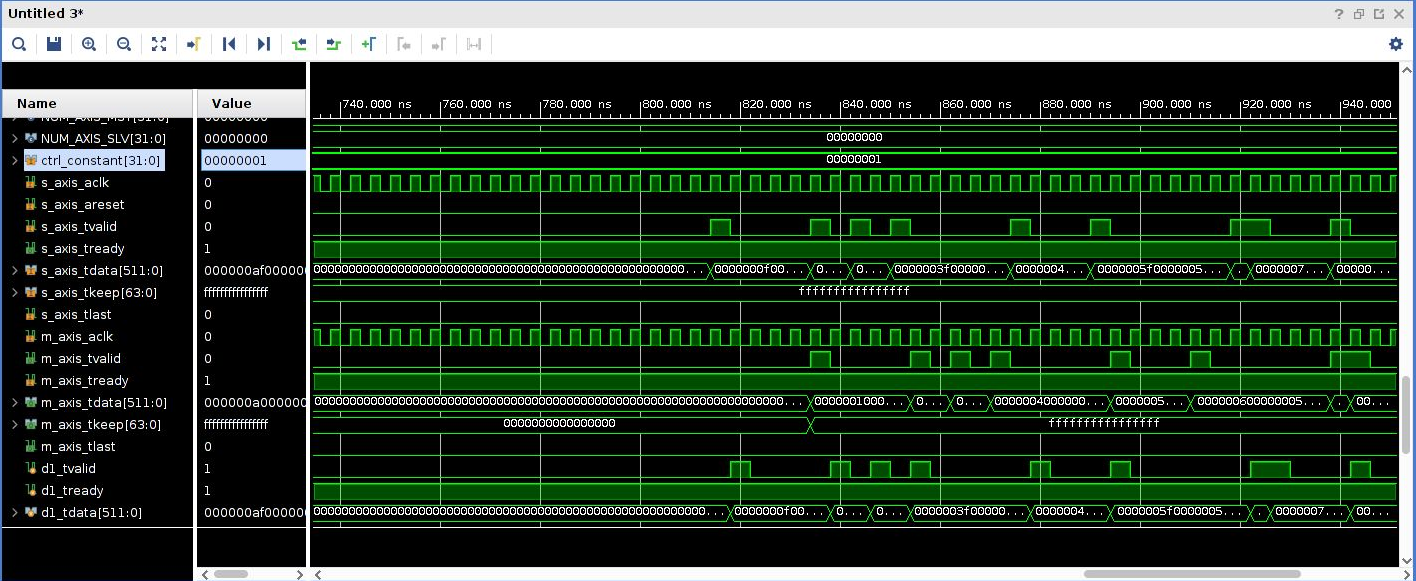
\includegraphics[scale=0.5]{images/diagram_increment_1}
		\caption{Транзакция записи результата инкремента данных на шине AXI4 MM}
		\label{png:increment}
	}
\end{figure}